\documentclass[
%bachelor, % Master version, default: Bachelor
%cover,  % Custom cover page, must be provided as an coverpage.pdf in A4 size
        % Default: HiØ standard thesis titlepage
%word,   % Word-like paragraph formatting, no indentations, air between paragraphs
        % Default: As all documents are formatted, except those made with default M$ documents
%sans    % Standard HiØ font: Source Sans Pro
        % Default: Computer Modern, designed by Donald Knuth.
]{thesistemplate}

\usepackage[british]{babel} % Add this if you use another language
% For available languages and their codes, see https://ctan.org/pkg/babel-contrib
\usepackage{lmodern}
% For those who needs code listings
%\usepackage{listings}
\usepackage{graphicx} % DO NOT CHANGE
%\renewcommand{\lstlistlistingname}{Kode} % If you are using another language, you need to specify the corresponding "Code List" title

%Metadata, to appear on the half-title page (and the coverpage, if not a custom cover is provided), to be changed by you:

\doctype{Bachelor Thesis}
\group{BO21-G27}
\department{Department of Information Technology}
\affiliation{Østfold University College}
\place{Halden, Norway}
\title{Advanced Image Recognition and AI Training} % Main title
\subtitle{Text extraction with machine learning}
\author{
    Joakim S. Aarskog,\+
    Sondre Lillelien,\+
    Sander Riis
}


\RequirePackage{glossaries}
\makeglossaries


\newglossaryentry{ML}
{
    name=Machine Learning,
    description={Machine Learning}
}

\newglossaryentry{API}
{
    name=Application Programming Interface,
    description={}
}
\newglossaryentry{HIOF}
{
    name=Østfold University College,
    description={}
}
\newglossaryentry{HRM}
{
    name=Human Resource Management,
    description={}
}
\newglossaryentry{OCR}
{
    name=Optical Character Recognition,
    description={}
}
\newglossaryentry{AWS}
{
    name=Amazon Web Services,
    description={}
}
    % OPTIONAL, goes with \printglossaries at the end
\begin{document}

\maketitle          % DO NOT CHANGE
%\makehalftitle      % DO NOT CHANGE
\frontmatter        % All stuff before Introduction: DO NOT CHANGE

\chapter*{Prerequisites (Optional)}
The reader should at least have a basic understanding of programing.
\newline
.Net
\newline
Machine Learning
\newline
Database

\input{abstract}
\input{acknowledgments}
%\chapter*{Prerequisites (Optional)}
The reader should at least have a basic understanding of programing.
\newline
.Net
\newline
Machine Learning
\newline
Database
   % OPTIONAL

\tableofcontents    % DO NOT CHANGE

\listoffigures      % OPTIONAL
%\listoftables       % OPTIONAL
%\lstlistoflistings  % OPTIONAL

\mainmatter  %Setting the format and layout for all the stuff from Introduction and on: DO NOT CHANGE

% Your chapter files

\chapter{Introduction}
\label{ch:intro}
A lot of companies have employees that travel in their work.
This travel is usually funded by their employer.
In order to keep track of all the transactions generated by this travel, the company will store the receipts from the transactions in order to refund their employees for their purchases.

Going through these transactions manually is time-consuming and labor intensive.
Because of this, creating an automated solution for extracting the data contained in these receipts will effectively reduce the amount of manpower and manhours required by the company.
This aim of this project is to explore and discuss these automated solutions.

\section{Background and motivation}\label{sec:background-and-motivation}
\subsection{Project Group}\label{subsec:project-group}
\textbf{Joakim Aarskog} is a 24-year-old computer science student at Østfold University College.
He has an interest in technology and photography.\\
\\
\textbf{Sondre Lillelien} is a 26-year-old computer engineering student at Østfold University College.
Interests include technology, engineering and AI.\\
\\
\textbf{Sander Riis} is a 23 years old computer science student at Østfold University College.
He likes to develop programs and learn about new technology.

\subsection{Employer}\label{subsec:employer}
The employer for this project is Simployer AS, a tech company that specializes in Human Resource Management (HRM).
They deliver HRM software to 15.000 customers and have over 1.2 million users in Norway and Sweden.
Simployer is passionate about giving other employers and their employees the tools to be able to effectively organize themselves.
Simployer is a sizable company with over 250 employees, and a history going back 35 years.
Our main contact in Simployer is Flemming Ottosen, their CTO.

\subsection{Problem statement}\label{subsec:problem-statement}
As Simployer delivers HRM software to many Scandinavian companies, they have a large database containing receipts generated by their employees.
These documents are stored in an unorganized manner, making manual validation of these documents difficult and time-consuming.
The documents are typically in the form of an image of a receipt taken with a mobile camera.
The documents lack metadata, which makes searching through them to find a specific document difficult.
Simployer would like a way to organize this data automatically and attach relevant metadata to the documents.
This metadata includes the price of the transaction, the company the service was purchased from, and the date of the transaction.
In addition to attaching metadata to existing documents, Simployer would like to automatically generate and attach metadata to new documents coming in to their database.

\subsection{Motivation}\label{subsec:motivation}
Artificial intelligence and machine learning is a rapidly growing field in computer science.
The biggest obstacles that AI and ML faced in the past was a lack of computing power and a lack of data.
In today's world, both of these obstacles have largely been overcome, as computing power keeps growing and data is a more abundant resource than ever.
The motivation for this thesis is to take advantage of this abundance of computing power and data to solve real life problems.

\subsection{Objectives}\label{subsec:objectives}
The objectives for this thesis are:
\begin{description}
    \item[Objective 1] To create a machine learning model that can identify desired data in an image of a receipt.
    \item[Objective 2] To have the machine learning model be capable of improving it's performance when new data is acquired.
    \item[Objective 3] To develop an API that can deliver data to the machine learning model and fetch the results.
\end{description}

\subsection{Method}\label{subsec:method}
The aim of the thesis has pivoted somewhat since the start of the project.
Originally the goal was to create a machine learning model that can correctly identify desired data from a large variety of images types with different quality.
The goal is still to create such a model, but more focus will be put into the learning module, with less focus put into being able to work with a large variety of images.

The methods used for this thesis are the following:
\begin{compactitem}
    \item Deep learning literature research
    \item Text analysis and text extraction articles
    \item Clearly defining the scope and objectives of the thesis
    \item .NET Core articles
    \item Workflow management in Jira
\end{compactitem}

\subsection{Deliverables}\label{subsec:deliverables}
The following items should be delivered by the projects end-date:
\begin{compactitem}
    \item A thesis report detailing the entire project
    \item A machine learning model that can extract desired data from the images it is given.
    \item An API that can deliver images to the ML pipeline and request the results of data extraction done on the images.
\end{compactitem}

\section{Report outline}\label{sec:report-outline}
Chapter 2 explains the thesis topic and scope of the project in detail.
In addition, the methods used to complete the work, along with literature the work is based on will be included here.

Chapter 3 provides a detailed walkthrough of how the project is designed.
The design is made to efficiently and correctly tackle the problem statement.

Chapter 4 describes the implementation of the project.
This includes how the project group chose to implement the design discussed in previous chapters, and the research methods used to arrive at design decisions.

Chapter 5 presents the results the project group's work in an objective manner.

Chapter 6 discusses the results discovered in chapter 5.
This includes how the results differ from what was expected, how the findings might be relevant to the thesis' field of study, etc.

Chapter 7 concludes and summarizes the thesis in a manner that can be read by someone who did not read the entire report.






\cleardoublepage
\chapter{Analysis}
\label{ch:analysis}

This chapter describes the practical and theoretical foundation of your project.
Basically, there are two aspects you should focus on, your research topic, and related work (literature and projects).

\section{Research topic}\label{sec:research-topic}

Our project is to create a solution that uses text recognition on an image and extracts the relevant data.
This solution will allow the user to take a picture of a receipt with their phone.
Then the information on the receipt will be extracted and analysed and automatically sorted into the database.
We are aiming for extracting 3 key details from the receipt: Date, Total amount(money) and understanding the type of receipt(like if it is a taxi receipt).

The app will consist of two main parts: The OCR(optical character recognition), and the model that reads the data.
We are going to use a free open source OCR, named Tesseracts.
The OCR is what will allow us to extract text from the images.
This OCR will send all the text that is on the receipt in the form of an array to the model.
The model will then decide what information is the correct data to extract and keep.

With the app we also need to include an API that will talk with the app and talk with Simployers server.
This API gets the data from the model and will prompt the information that is selected for the user for a final
validation, before sending it to the Simployer database.
This will allow Simployer to easily search in the database based on the metadata that was extracted.

Here you will describe the thesis topic in sufficient detail to work out the details of your project, so that the reader gets a perfectly clear picture of the settings of your project.
It is important to define your scope, and perhaps narrow down a broad subject.
Also, if there are such, describe constraints and requirements you need to follow.

If your work is part of a larger project, or if you are cooperating with an external company or research institute, this is the place to tell the reader about that.

\section{Tools}\label{sec:tools}
\subsection{Google Cloud Vision API}\label{subsec:API_Google}

Google Cloud Vision API contains a well optimised OCR and good variety of detection.
The detection features includes:

\begin{figure}[h]
    \center{\includegraphics[width=1\textwidth]{Images/googleAPI_features}}
    \caption{Overview of features (list from https://cloud.google.com/vision/pricing)}
    \label{fig:Features}
\end{figure}

We can see that Google API offers everything from text recognition to landmark location and crop Hints.
The Google API is know to be industry leading in the field, so this comes as no surprise.
This API will have almost everything you need to develop an application with text recognition.

The API also has a lot of features in their beta version which is not included in the list above.
\clearpage


\begin{figure}[h]
    \center{\includegraphics[width=1\textwidth]{Images/googleAPI_prices}}
    \caption{Overview of features (list from https://cloud.google.com/vision/pricing)}
    \label{fig:Prices}
\end{figure}

Google is the best in the field, but they are also the most expensive API to use.
The prices are calculated for each 1000-request.
This means that you are getting the first 1000-requests free and then you will need to play 1.5\$ for each 1000-request you do on for example text detection.
If you have a request size of 50.000-requests this will be 49*1.5\$ = 73,5 dollars (620 NOK).
This will reset every month.

\subsection{Amazon Textract}\label{subsec:API_Amazon}

Amazon's AWS hosts a service called Textract.
This cloud-based service lets you upload an image to their text recognition software.

\textbf{Detect Document Text API}
This feature is the classic OCR feature that will extract text from a document.
Amazon will charge you 0.0015\$ per page (1.50\$ per 1000) for the first million pages, when you exceed 1 million the price wil go down to
0.0006\$ per page (0.6\$ per 1000)

\textbf{Table Extraction}
This is an improved version of Detect Document Text API. This will group the text in tables.
This is helpful with structured data, such as financial reports.
Amazon will charge you 0.015\$ per page (15.0\$ per 1000) for the first million pages, when you exceed 1 million the price wil go down to
0.01\$ per page (10\$ per 1000)

\textbf{Form Extraction}
This detects key-value pairs in documents, for example if your document has a field named "first name" it will pair it will Mike.
This way "first name" would be the key and "Mike" would be the value.
This makes it easy to either sort it into a database or reuse the values in variables.
With normal OCR the relation is lost.
Amazon will charge you 0.05\$ per page (50\$ per 1000) for the first million pages, when you exceed 1 million the price wil go down to
0.04\$ per page (40\$ per 1000)

\textbf{Analyze Document API}

This is a combination of the tables and forms extraction
Amazon will charge you 0.065\$ per page (65\$ per 1000) for the first million pages, when you exceed 1 million the price wil go down to
0.05\$ per page (0.50\$ per 1000)

Note that Amazon changes their pricing on the region you are in (you might want to check the price for your region), they also do not include a free 1000 scans per a month.

\subsection{Open source OCR}\label{subsec:Open source}
The one open source OCR that is looked at as the best is tesseract.
This was first produced by HP in the 80's and later made open source in 2005 and funded by google since 2006.
Most OCR programs today are build on this, like google cloud vision API. This is our 3rd and final option.
This will require us to code and make an OCR for ourself.
This is no problem if you only work with pdf and other document types like this.
This requires little to no pre-processing or tuning.
The problem starts when you are going to extract text from a picture.

You will need a lot of pre-processing and tuning to make this even work, not to mention read correctly.
This is because OCR's need good contrast and little to no noice in the pictures.
Another problem is curved text, like in a book.
This might be the hardest ting to solve.

\textbf{Scaling the image}
You should try to scale the image in a size between 300dpi and 600dpi.
Anything less will make it unreadable for the OCR and anything more will just take up processing power.

\textbf{How to create contrast}


First you will have to transform the image from RBG into a grayscaled image.
This image can then be used to make a threshold for the image.
Adaptive threshold is a built in function in openCV, that breaks the image into different sections.
There it tries to find the optimal threshold for the local part of the image.
This means that it removed noise and optimises blur in the image.
This sounds very good, but we have found that a combination of global threshold and something that is called Otsu's threshold (threshold that is the same for the whole image).
Is the best way to make a threshold you also will need to use Gaussian blur on the image before you use the threshold on the image.
this blur function will try to remove as much "grain" on the image as possible.

\textbf{Remove background noise}
There is always noise in the image.
Removing noise in the background is very important to improve readability.

\textbf{Straighten the image}
It is very important to rotate the image to a horizontal level.
The OCR does not read text that is tilted.

\textbf{Edge detection}

\section{Summary}\label{sec:summary}

Sometimes, in particular when the chapters are quite long, they are ended with short summaries.

\chapter{Design}
\label{ch:design}

\begin{figure}[h]
    \center{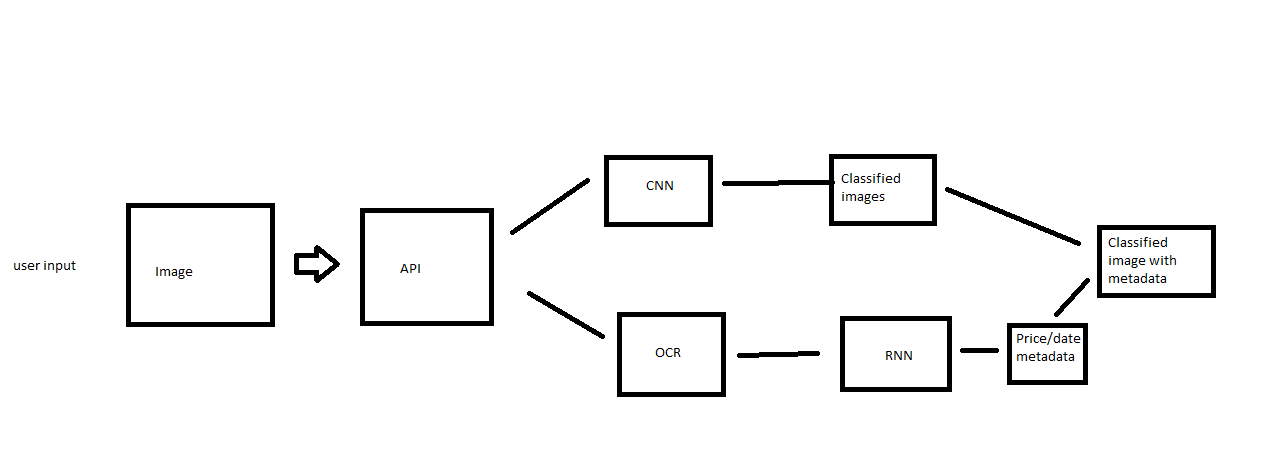
\includegraphics[width=1\textwidth]{Images/pipeline}}
    \caption{Graphic illustrating the project pipeline (PLACEHOLDER)}
    \label{fig:figure3}
\end{figure}
The project is designed to be able to take an input image of a receipt sent over http, and provide metadata to that image based on it's contents.
This metadata includes the company name that issued the receipt, the date the receipt was made, and the price of the purchase.
In order to transfer the image to our machine learning models, a .NET API is used.

The API exposes several endpoints that allows for saving an image and a receipt to a database.
The API is also connected to the CNN and OCR module.

We have decided to split up the metadata extraction into two separate parts;
a Convolutional Neural Network for image classification and a Recurrent Neural Network for natural language processing.

The CNN will take an image as input, and decide which company issued that receipt based on previous training data.

The RNN will take text as input.
In order to extract the text from the images, an open-source OCR is used.

Finally, the outputs of the CNN and RNN and combined and provided back to the user.
This pipeline is illustrated in figure 3.1

\section{API}\label{sec:API}
The API is used as the connection point between the different modules, it sends and receives data through the pipeline.
The user sends in an image via a website and the API handles the request and sends the data to the CNN and the OCR\@.

When the data has been processed through the CNN and OCR, the API sends the data back to the
user.

\section{Dataset}\label{sec:dataset}
In order to train our neural network models, Simployer provided us with a sample of images from their database.
This dataset includes 1194 images of receipts taken with mobile cameras and generated pdfs from online sales.

\begin{figure}[h]
    \center{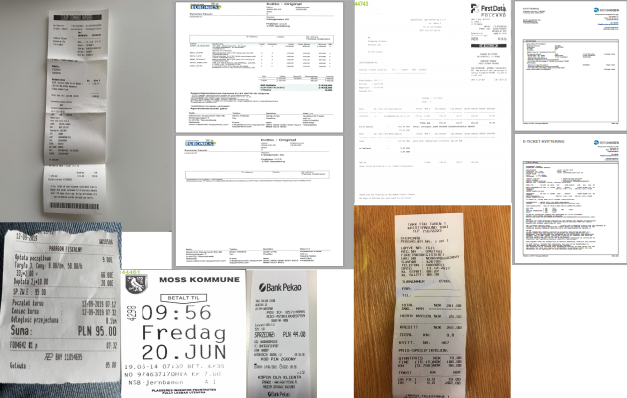
\includegraphics[width=1\textwidth]{Images/exampleimages_raw_resized}}
    \caption{Examples of the images found in the dataset provided by Simployer}
    \label{fig:figure3.2}
\end{figure}

This dataset is not labeled, which means we have to manually label the data we are going to use to train our networks.
Because of the large variance of different types of companies in this dataset, creating labels for all of them would be very time-consuming.
Instead of labeling them all, we decided to restrict ourselves to the three most common receipts found in the dataset.
This means the amount of images we can use for training is greatly reduced, so in order to combat this, we used data augmentation software to generate more images.
This is discussed in greater detail in chapter 4.

\section{Pre-processing}\label{sec:pre-processing}
A CNN does not require images of large resolution in order to accurately classify an image.
In addition, training the network with large resolution images take significantly longer.
Because of this, all the images that are going to be fed into the CNN are downscaled.
This also solves the problem of images being of different sizes, as the CNN requires all the images to have the same size.

\begin{figure}[h]
    \center{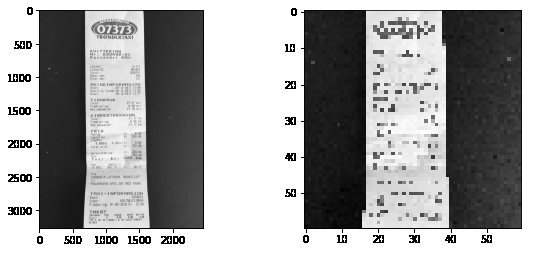
\includegraphics[width=1\textwidth]{Images/beforeafterrescale}}
    \caption{Before and after image rescaling}
    \label{fig:figure3.3}
\end{figure}
While the text in the image is now completely unreadable, the CNN will have no issues telling images in this format apart from each other.

\section{Convolutional Neural network}\label{sec:CNN}
As stated previously, we are using a CNN as an image classifier in order to determine which company issued the receipt.

\begin{figure}[h]
    \center{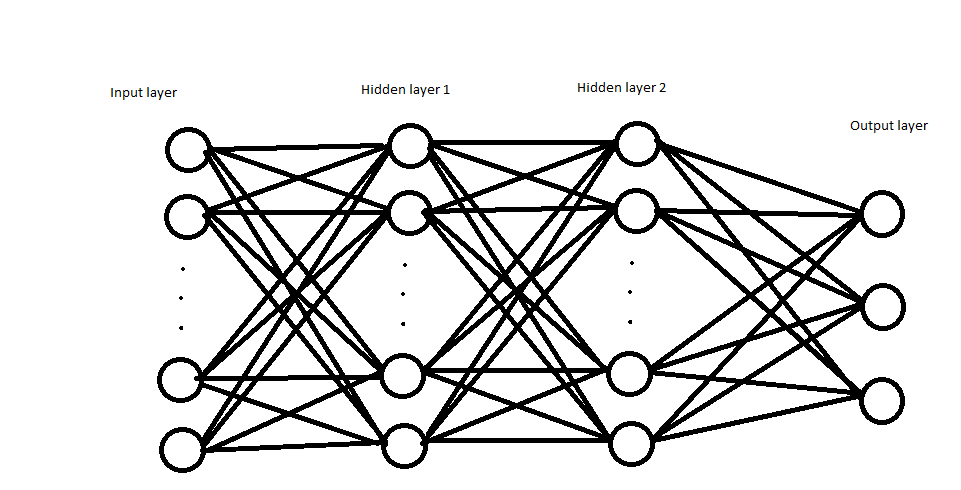
\includegraphics[width=1\textwidth]{Images/cnnplaceholder}}
    \caption{Graphic illustrating the Convolutional Neural Network (PLACEHOLDER)}
    \label{fig:figure3.4}
\end{figure}

Figure 3.3 illustrates the layout of our CNN.
The input layer takes the pixel value of the image.
Because of this, the number of nodes in the input layer has to be equal to the amount of pixels in the image.
The output layer has three nodes, one for each type of receipt the network is trained to classify.

We are using a supervised learning-model to train our network.
Because of this, the training data has to be labeled.
This labeling can be labor intensive if the dataset you are labeling is large.
Since we started with a very small amount of images before the use of data augmentation, it is a small task.

\section{Optical Character Recognition}\label{sec:OCR}
In order to extract the text found in an image, we are using the open-source OCR software Python-tesseract.
Python-tesseract, or Pytesseract for short, utilizes Google's Tesseract-OCR engine.

When metadata for a particular image is requested by a user, the API will provide our implementation of Pytesseract with an image.
Pytesseract will take this image as an input, and can provide outputs in various formats like xml or pdf.
We will be using the output in string format, as this will serve as the input to our RNN model.
Once Pytesseract has completed the text extraction, the output string is then fetched by our API to be provided to our RNN model.

\begin{figure}[h]
    \center{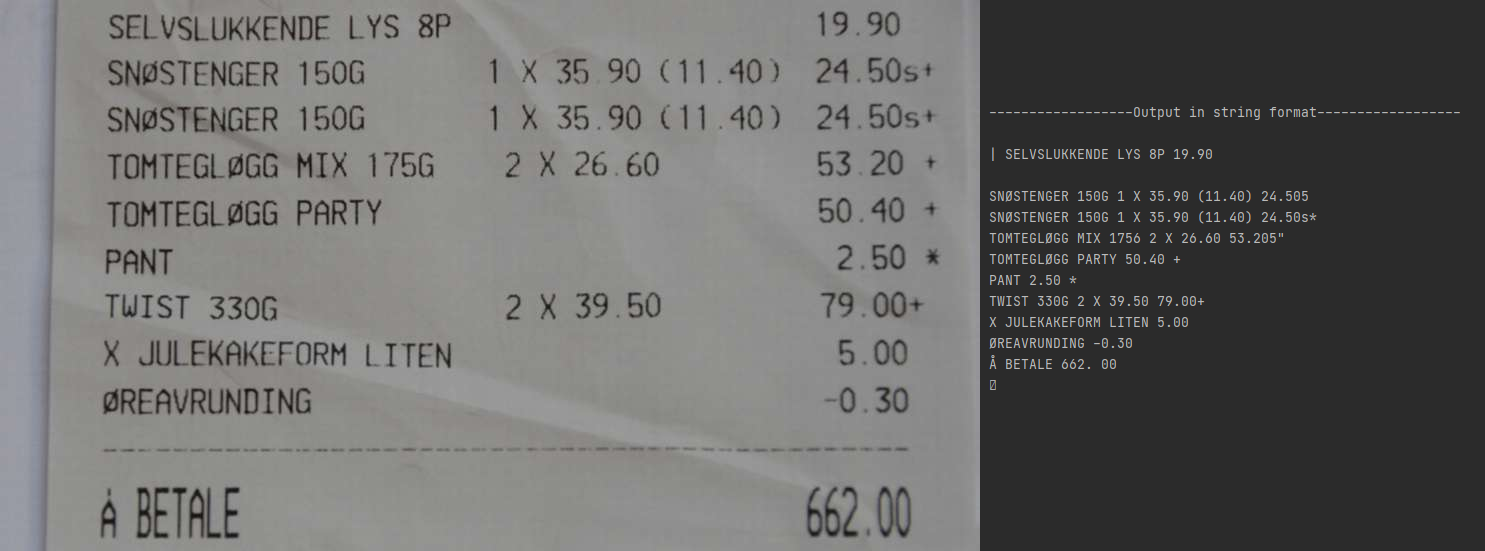
\includegraphics[width=1\textwidth]{Images/ocr_before_after}}
    \caption{Example output of pytesseract with a test image}
    \label{fig:figure3.5}
\end{figure}

\section{Recurrent Neural Network}\label{sec:RNN}


\cleardoublepage
\chapter{Implementation}
\label{ch:implementation}
Chapter 4 describes the implementation of the thesis.
This includes how the thesis group chose to implement the design discussed in previous chapters, and the research methods used to arrive at design decisions.

\section{REST API}\label{sec:REST API}

The API is a REST API coded in C\# with .NET.
REST stands for REpresentational State Transfer and is a software architecture style.
For the API to be considered a REST API it has to follow some set guidelines and principles.

The API consists of 4 different modules: The API endpoints, DataAccess,\\
DataAccess.Maintenance and Model.

\textbf{API endpoints} contains the controllers which handles the routing and requests.
There are three controllers, one for receipt, one for image and one for connecting to the machine learning API\@.
They receipt and image contain the methods GET, POST, PUT, and DELETE\@.
While the machine learning only contains on  for posting a picture.

In ImagesController the POST method uses the ImageDTO object.
It initializes a new Image object, and populates the corresponding data.
To set the image data, it serializes the image data from the DTO, and uses this data to for the image data.

\textbf{DataAccess} contains the DataContext for the database.
For the sake of simplicity, we have decided to utilize a local database.

\textbf{DataAccess.Maintenance} contains the migrations for the project.
This is to make it cleaner and to have a console app where it is possible to update the database without having to run the API\@.

The \textbf{Model} module contains the different models we use.
There is one for receipts and one for image, there is also a data transfer object for image.
The DTO is an object that carries data between processes and makes it more efficient by doing it in only one call.
This is done by aggregating the data instead of sending it one by one.


\section{ML API}\label{sec:ML API ch4}
The ML API is created using Flask.
This has one POST route that takes in an base64 string and converts it to an image and sends it to CNN and OCR for
processing.
The data is then returned to the .NET API

\section{Web solution}\label{sec:Web solution}

The web solution is made with React in JavaScript.
The purpose of the web solution is to give the user an interface where they can upload an image of a receipt.
And get the corresponding data from the image, and then send in the receipt with the data from the image.
This is to make the process of entering the data less time consuming.

When the user uploads an image, the web solution sends a POST request to the API, then the API saves the image to
the database.
When the image is saved, the image is sent to the OCR for text recognition.
If the output makes sense the data is returned and displayed to the user.
Then if the returned data is correct the user can then upload the receipt to the database.

\section{Dataset}\label{sec:dataset2}

As mentioned previously, dataset provided by Simployer consists of 1194 unlabeled images and PDF's.
However, the variance of the types of receipts in the dataset is very large.
When attempting to label the data with the corresponding company name, the amount of different companies were very large.
Because of this, we end up with a very small amount of images of each type after labeling them.
We decided to use the 3 most frequent companies, with the third most frequent company occurring only 19 times.
At the end of this process, the amount of usable data was very small.
The original dataset of 1194 images has been filtered down to 91 images, split into three different types of receipts.

\begin{figure}[h]
    \center{\includegraphics[width=1\textwidth]{Images/exampleimages}}
    \caption{Examples of labeled images}
    \label{fig:figure4.1}
\end{figure}

\section{Pre-processing}\label{pre-processing}

\subsection{Aligning}\label{aligning}

The first thing we make sure to do in our OCR is aligning the images.
This is needed because an OCR can't reed skewed images.
This means that we need to horizontal align the text as well as possible.

\subsubsection[aligning]{Matching}

Matching is a good way of having a dynamic aligning algorithm.
We have template images for all the different receipts types (in this case 3 images).
What the matching algorithm does is to look through the receipt you feed it and see if it has any "mathces" with the template one.
It then calculates how much it needs to skew the image in a given direction, to make it aligned with the template version.

\begin{figure}[h]
    \center{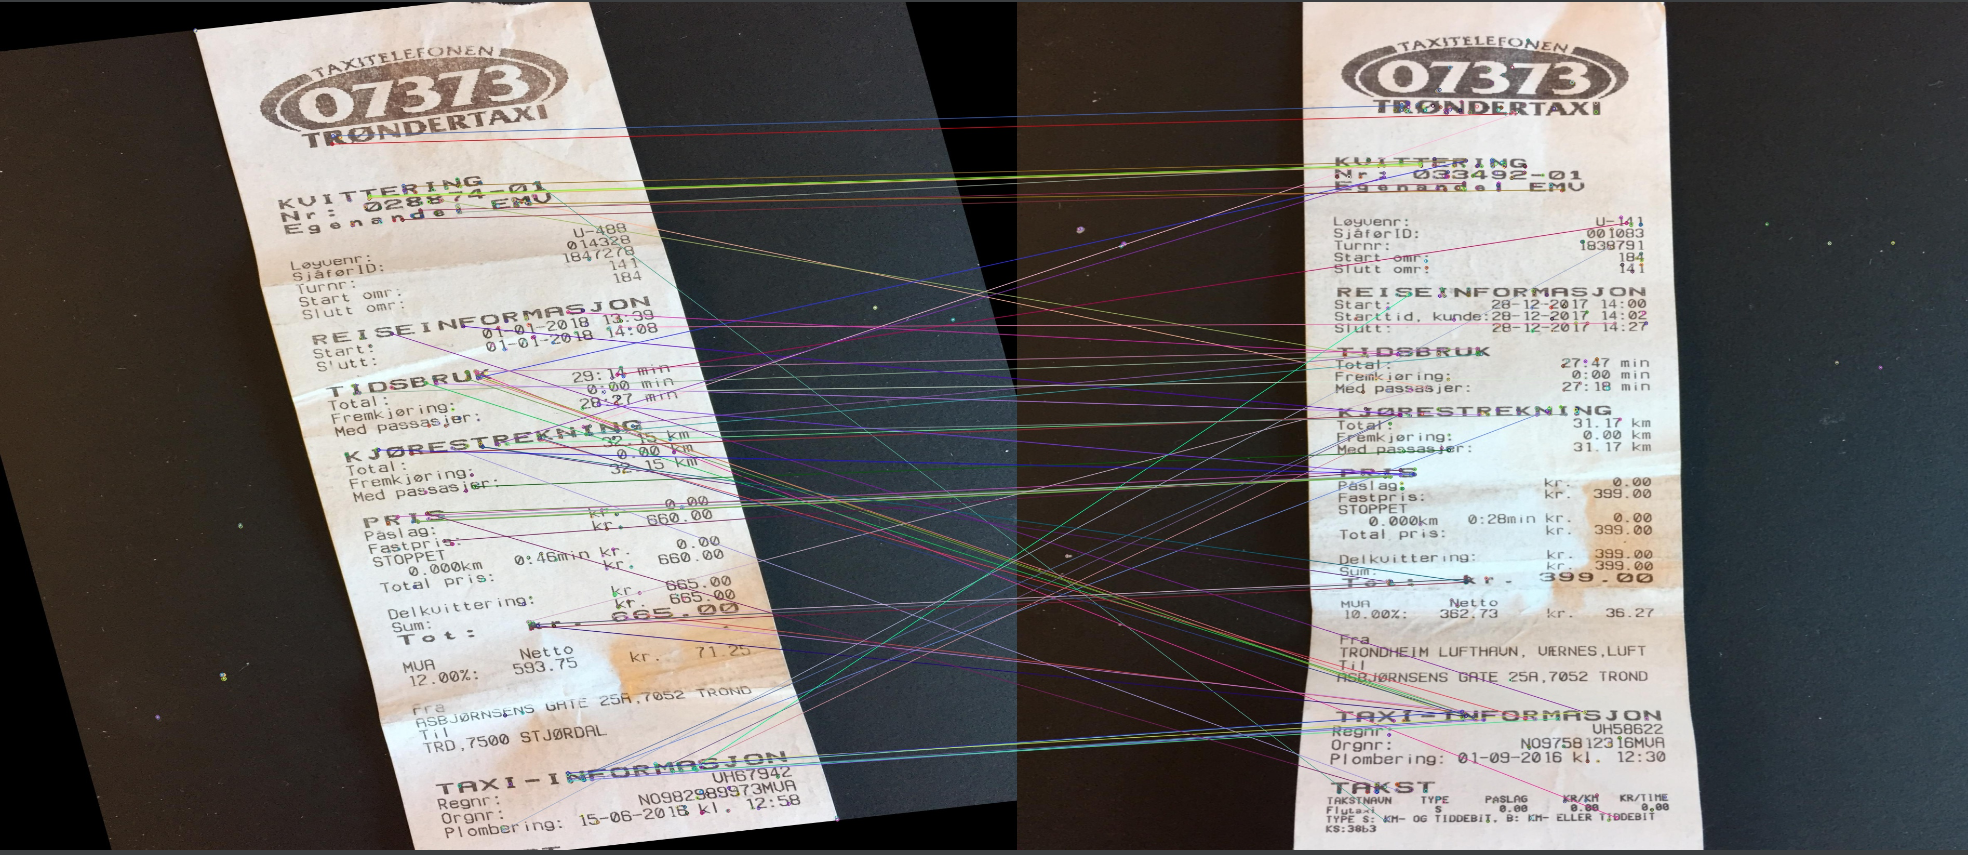
\includegraphics[width=1\textwidth]{Images/match_image.png}}
    \caption{Finding matches between a given image to a template}
    \label{fig:figure4.2}
\end{figure}

In the image above you can see the algorithm finding matches between a Trøndertaxi receipt from two different years.
Yes, these recipes is almost identical.
Making this functionality dynamic for almost all receipts should be possible, (no evidence for this) by having a pool of template receipts.
Then you can have a CNN check which receipts are the most similar and use the highest scoring receipt as the template image for any given receipt.

\subsection{Data augmentation}\label{data augmentation}
Because of the low amount of images in the filtered dataset, data augmentation has to be done in order to give us enough images to be able to effectively train the CNN.
We used an open source data augmentation tool for images for this task LINK.
The augmentor takes a directory of images and applies a series of transformations on the images like scaling, skewing and rotating.
This creates copies of the images with slight differences, increasing the size of our dataset.
After applying enough transformations, the size of the dataset grew from 91 images to 1500.

\begin{figure}[h]
    \center{\includegraphics[width=1\textwidth]{Images/example_augmented}}
    \caption{Original image on the left, along with generated images from blur and rotation transformations}
    \label{fig:figure4.2}
\end{figure}

\subsection{Image preparation}\label{imgprep}
Many of the images in the dataset are taken in different resolutions.
In order to prepare the images to be passed forward to the CNN model, the images resolution is rescaled to 60x60 pixels.
This significantly reduces the training time required by the network with minimal to no loss in accuracy.
The images are also converted to grayscale instead of RGB.
This reduces the amount input nodes required by the network, as each pixel will have one value instead of three.

\section{Convolutional Neural Network}\label{sec:cnn}

Our CNN is implemented using Keras.
Keras is a library for tensorflow that allows for the creation of neural network models with only a few lines of code.
The model consist of an input layer, two hidden layers, and an output layer.
The input layer and first hidden layer are 2D convolutional layers with 32 and 64 filters.
The second hidden layer, and the output layer are dense layers, where the hidden layer has 64 filters and the output layer has 3 filters.
The activation function of the first three layers is Rectified Linear Unit (ReLU), while the output layer uses the sigmoid function.
Maxpooling2D is used to define a stride of 2.
This means that we take the biggest number with something that is called a max operation.
We combine the results to get a 2x2 max pool output, down from a 4x4 format.
As illustrated below.

\begin{figure}[h]
    \center{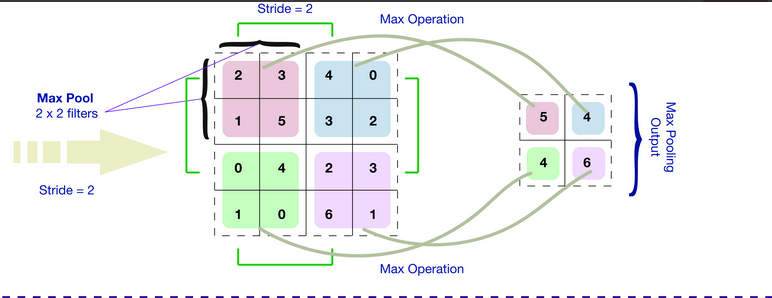
\includegraphics[width=0.8 \textwidth]{Images/maxpooling2D}}
    \caption{Overview for max pooling (Image from https://www.quora.com/What-is-max-pooling-in-convolutional-neural-networks)}
    \label{fig:figure6}

\end{figure}

We have also used batch normalisation with the default settings in the input and hidden layers of out model.
This means that the model is sharding the data in batches.
This in turn lets us train the model with a lot less training steps, and it gives us even better accuracy.
The last function we will talk about in the input and hidden layers are the dropout function.
This function will force the model to drop random filters during the training.
This will force an adaption in the model that makes it more versatile.
This is because the model can't just rely on one good path to carry its accuracy.
Therefore, it will end up with a more generic understanding of the data and avoid an overfitting.

\begin{figure}[h]
    \center{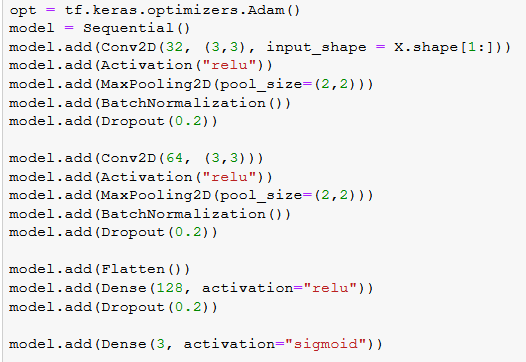
\includegraphics[width=0.8 \textwidth]{Images/CNN_model}}
    \caption{CNN model}
    \label{fig:figure4}

\end{figure}

In the compile function we defined we choose to use cross-entropy as our loss function.
Because this is the best for multiclass classification.
The optimizer is the standard adam optimizer.



\begin{figure}[h]
    \center{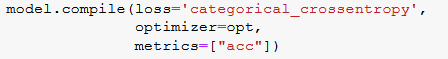
\includegraphics[width=0.8 \textwidth]{Images/CNN_compile}}
    \caption{CNN model compile}
    \label{fig:figure5}

\end{figure}


\section{OCR}\label{sec:OCR_implementation}

The first thing we did in the OCR was

\begin{figure}[h]
    \center{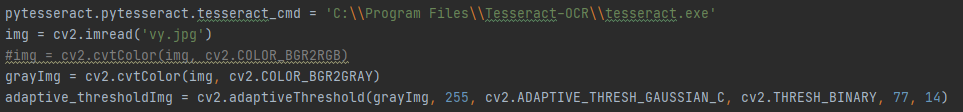
\includegraphics[width=0.8 \textwidth]{Images/OCR1}}
    \caption{CNN model compile}
    \label{fig:figure7}

\end{figure}

\begin{figure}[h]
    \center{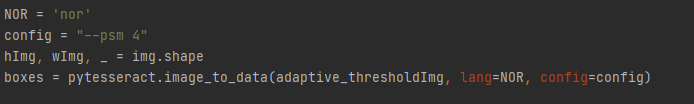
\includegraphics[width=0.8 \textwidth]{Images/OCR2}}
    \caption{CNN model compile}
    \label{fig:figure8}

\end{figure}

\begin{figure}[h]
    \center{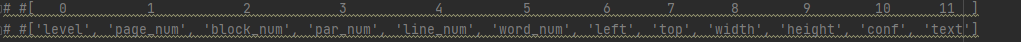
\includegraphics[width=0.8 \textwidth]{Images/OCR4}}
    \caption{CNN model compile}
    \label{fig:figure9}

\end{figure}

\begin{figure}[h]
    \center{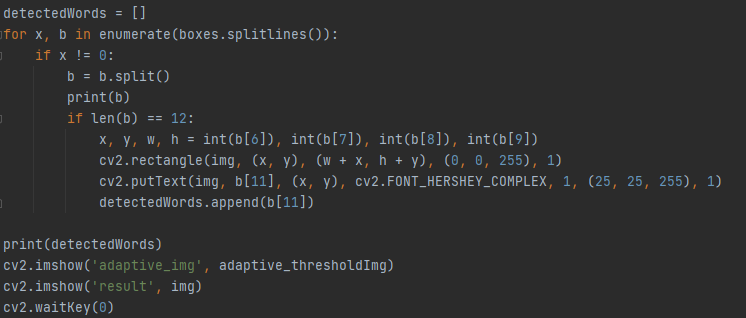
\includegraphics[width=0.8 \textwidth]{Images/OCR5}}
    \caption{CNN model compile}
    \label{fig:figure10}
\end{figure}


\chapter{Evaluation}
\label{ch:evaluation}
This chapter presents the results of the data extraction from receipts, as well as the results of each module.

\section{API results}\label{sec:api-results}
The implementation of our API's are made as a MVP\@.
This means that there is little to no validation on the input and the output, which means it only really works when
you send in the correct input.

\subsection{.NET API}\label{subsec:.net-api}

When the right input is sent in, the API functions as expected.
The input is an ImageDTO that comes from a POST request sent from the React module.
The image data from the ImageDTO is then correctly converted to a base64 string, which is then sent to the ML API through a POST request.

The result of the POST requests to the ML API is converted in to a receipt object and returned to the React module
where it is correctly displayed in their respective fields.

\begin{figure}[h]
    \center{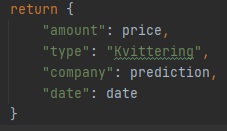
\includegraphics[width=0.5\textwidth]{Images/MLAPIreturnObject}}
    \caption{The result from the ML API}
    \label{fig:MLAPIreturnObject}
\end{figure}
\clearpage
\subsection{ML API}\label{subsec:ml-api}
The ML API takes in a base64 string from a POST request originating from the .NET API\@.
This string contains the image data, and is correctly converted to an image.
The image is then sent to the CNN and OCR\@.
From the CNN we get the company.
From the OCR we get the date, and a string, which is sent to Spacy and is used to get the price from the receipt.

The result of this is a json object with the corresponding data.
Shown in figure~\ref{fig:MLAPIreturnObject}.

\section{CNN results}\label{sec:cnn-results}
Many different CNN models with slight variations in their parameters were trained and tested.
Initially, the models had a low prediction accuracy, predicting the correct category about one third of the time.
Tweaking was done to the model by adding dropout, data normalization and max pooling.
Prediction accuracy then went up to around 95\% for most models.

\begin{figure}[h]
    \center{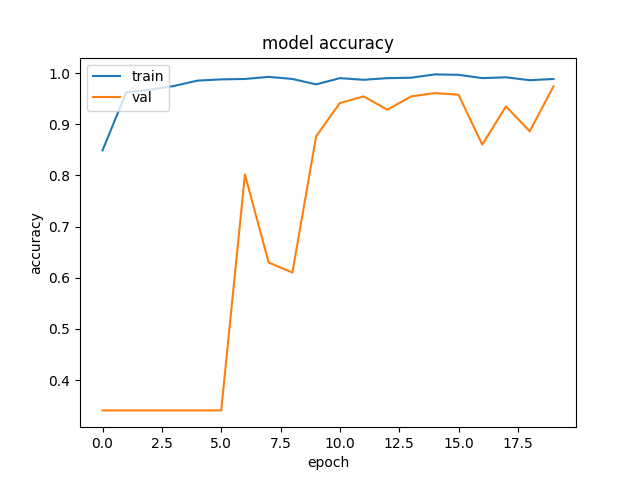
\includegraphics[width=0.8\textwidth]{Images/200modelaccuracy}}
    \caption{Training and validation accuracy for a model trained on 200x200 images}
    \label{fig:200modelaccuracy}
\end{figure}
\clearpage
Validation accuracy and loss are the two metrics we are using to determine the success of a model.
Figure \ref{fig:200modelaccuracy} and figure \ref{fig:200modelloss} shows how the model accuracy and loss are improving with each epoch of training.
A consistent theme when training our models was the validation accuracy and loss starting to radically improve between epoch 10 and 15.

\begin{figure}[h]
    \center{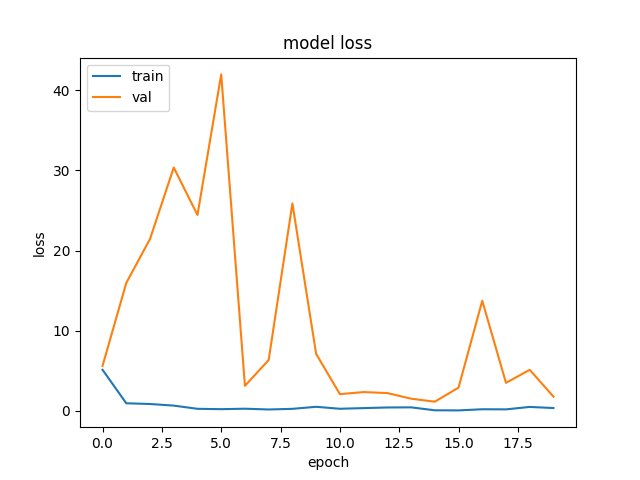
\includegraphics[width=0.8\textwidth]{Images/200modelloss}}
    \caption{Training and validation loss for a model trained on 200x200 images}
    \label{fig:200modelloss}
\end{figure}


\begin{figure}[h]
    \center{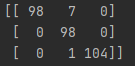
\includegraphics[width=0.3\textwidth]{Images/200confusion}}
    \caption{Confusion matrix for a model trained on 200x200 images}
    \label{fig:200confusion}
\end{figure}

A confusion matrix was also used to give some more insight into how the model was performing for each of the different categories it had been trained on.
Figure \ref{fig:200confusion} shows the confusion matrix generated from the same model as figure \ref{fig:200modelaccuracy} and figure \ref{fig:200modelloss}, using the same validation dataset.
The confusion matrix has three throws, one for each category of receipt the model has been trained to classify.
The diagonal of the matrix shows how many correct classifications the model made.
The rest of the fields shows how many incorrect classifications were made.
In figure \ref{fig:200confusion}, we can see that for the second category, all the predictions made were correct.
We can also see that most of the incorrect predictions were done on the first category, with 7 of the 8 incorrect predictions taking place here.

When trying to do predictions on a single image, the results were more inconsistent.
Predictions were made using images from the same dataset that it was trained on, with varying success despite good accuracy from validation during training.
For example, model A and model B might both have gotten validation accuracies over 95\%.
When tested on single images model A would always predict that category 1 was category 2, while model B would predict the categories correctly.

\section{OCR results}\label{sec:ocr-results}
Since our OCR implementation uses pre-defined templates to de-skew images, the output of our CNN plays a big part in whether the OCR will be able to extract text from the images.
When the CNN does not accurately predict the correct category for an image, the OCR de-skew will use the wrong image template, and the result of this de-skew becomes an image that is unusable.
This can be seen in figures~\ref{fig:scuffedmatch2} and~\ref{fig:scuffedmatchresult}.

\begin{figure}[h]
    \center{\includegraphics[width=0.85\textwidth]{Images/matchesscuffed2}}
    \caption{Input image (left) trying to match its content to the wrong image template (right)}
    \label{fig:scuffedmatch2}
\end{figure}

\begin{figure}[h]
    \center{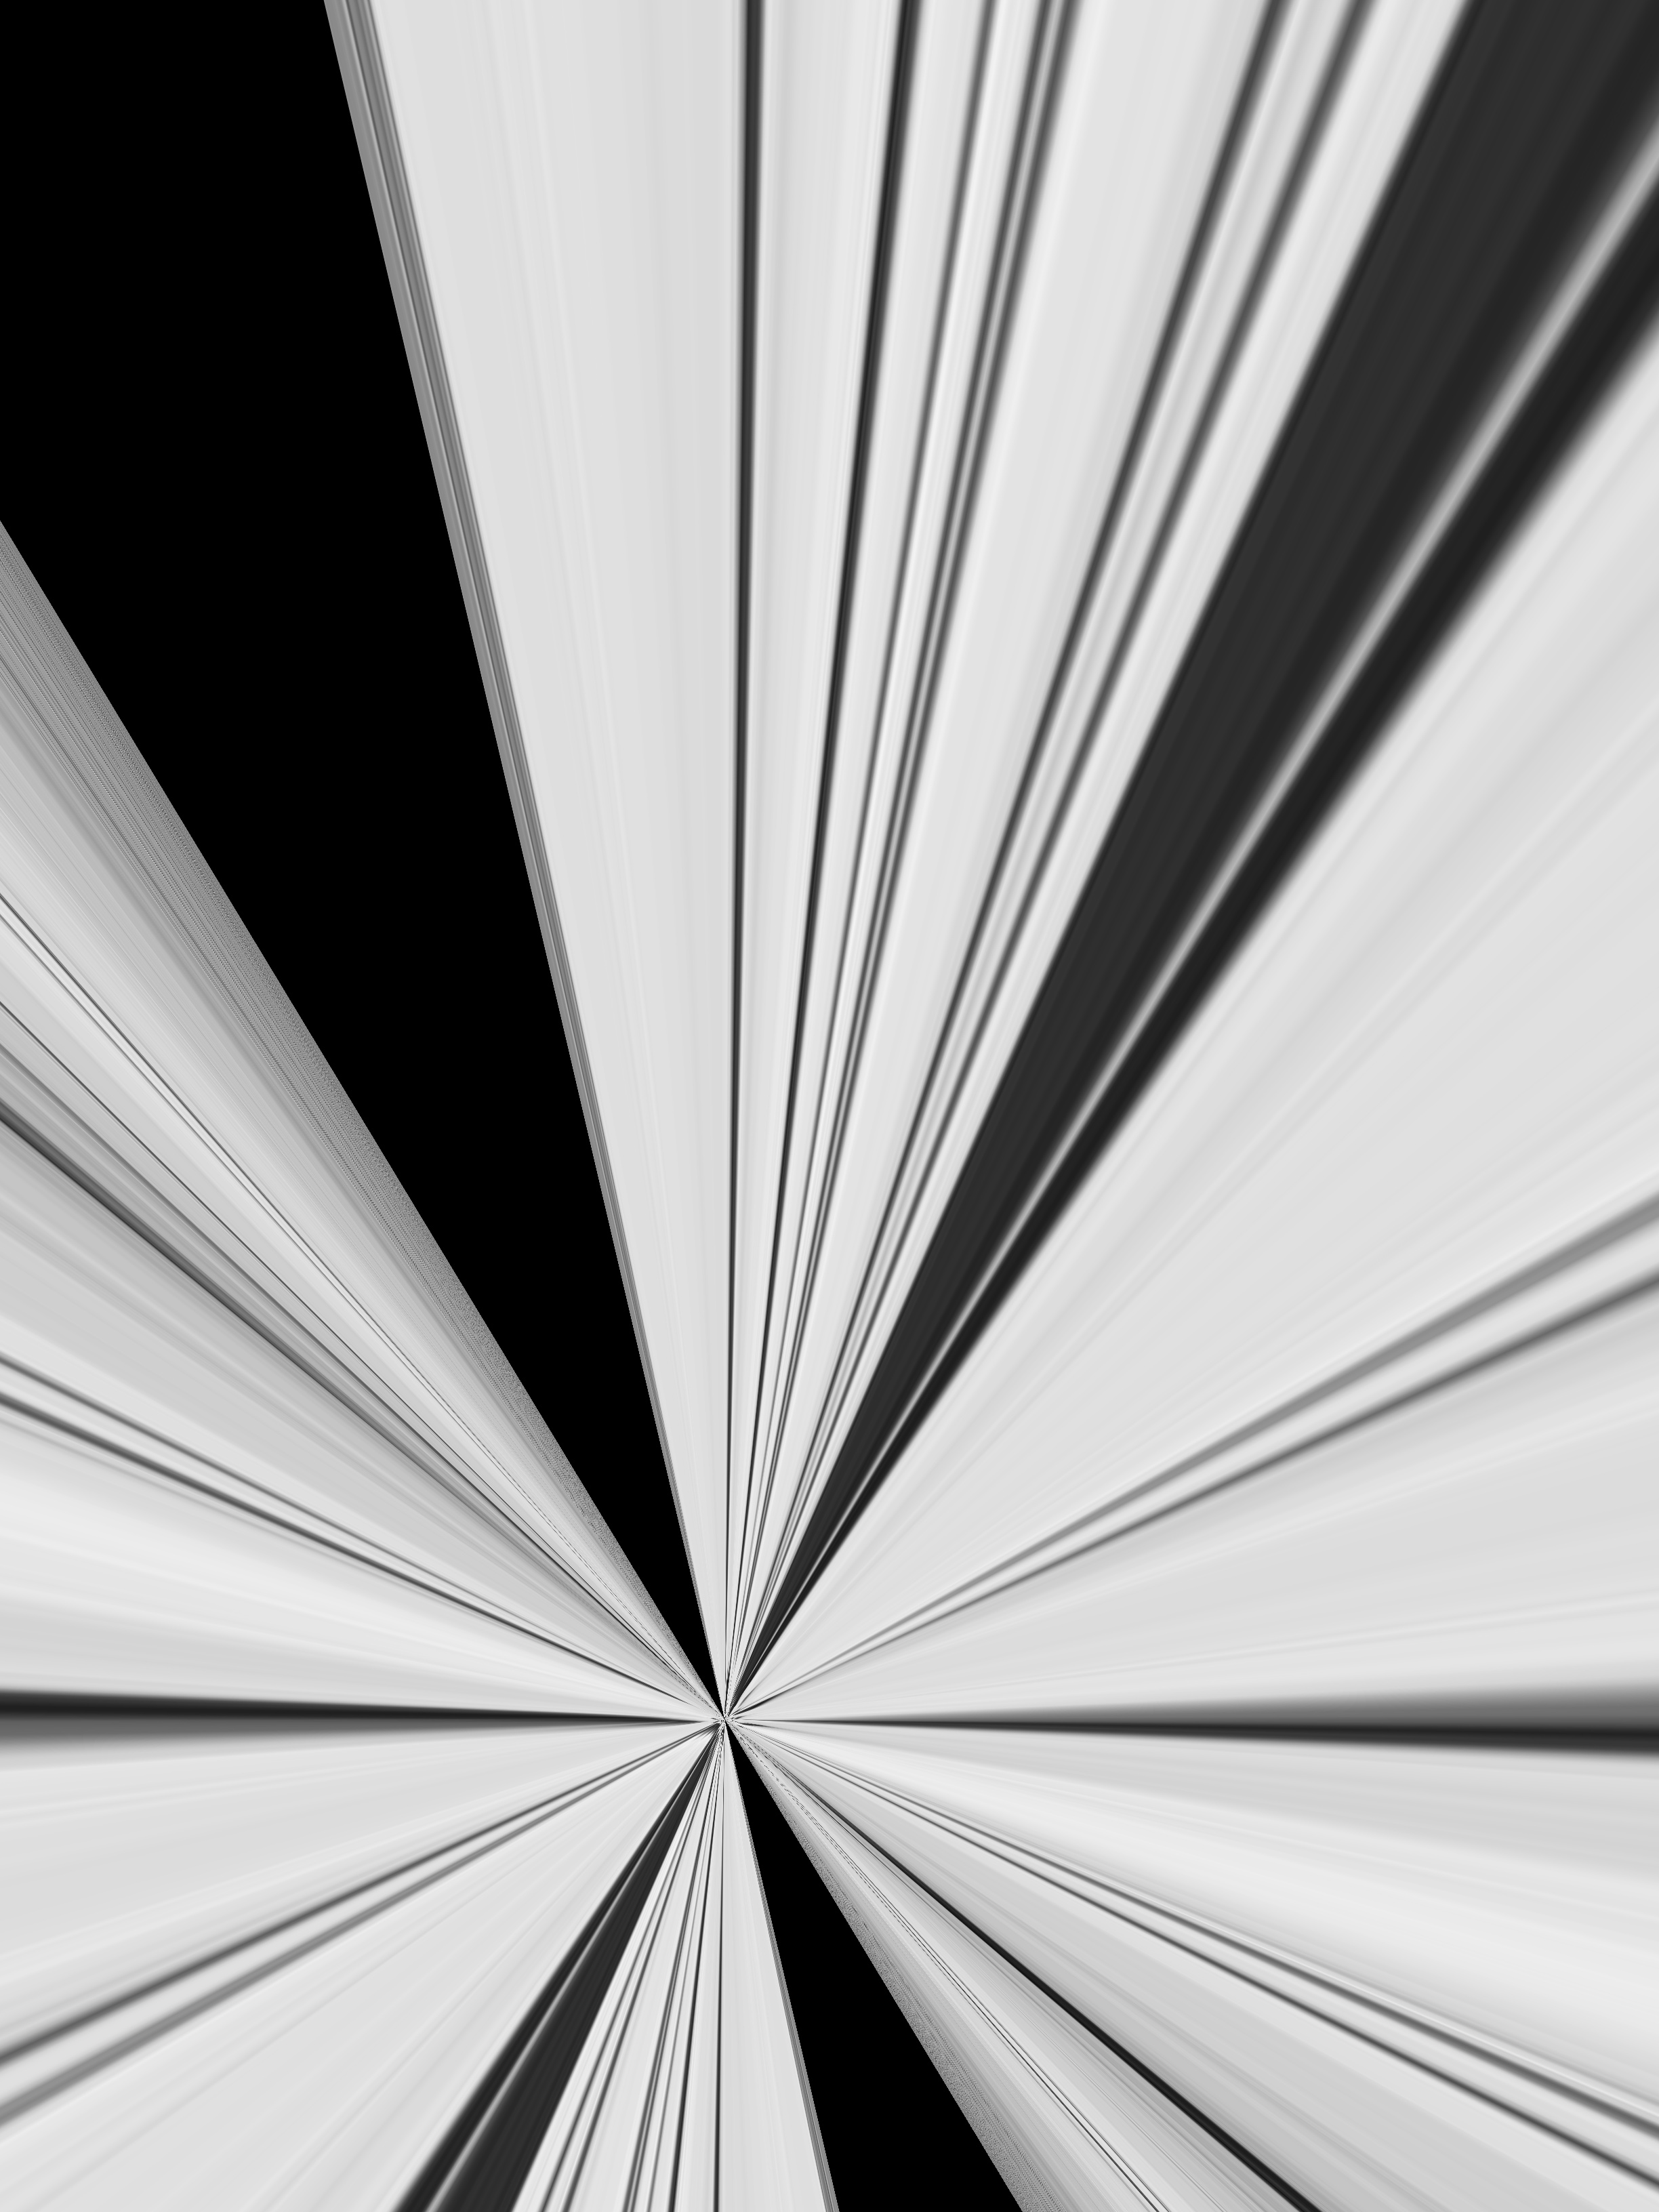
\includegraphics[width=0.3\textwidth]{Images/alignedscuffed}}
    \caption{Result of de-skewing when using the wrong image template}
    \label{fig:scuffedmatchresult}
\end{figure}

Because of this, the OCR module does not give any text output when the predicted category is not correct.
When isolating the OCR module from the other modules, or when the CNN predicts the correct category, the text output from our OCR module is mostly accurate.
However, small mistakes in the text extraction can lead to the wrong piece of data being extracted or not found at all.

\begin{figure}[h]
    \center{\includegraphics[width=0.6\textwidth]{Images/beforeafterpreprocess}}
    \caption{Before and after pre-processing}
    \label{fig:beforeaftepreprocess}
\end{figure}


Figure~\ref{fig:beforeaftepreprocess} shows the input image sent to the OCR on the left and the image after going
through pre-processing on the right.
Since the CNN made the correct prediction on what category of receipt this is, the de-skewing algorithm successfully straightened the image.
The figure also illustrates the binarization of the image, making the text easier to distinguish from the background.
An attempt to extract the text from the right-hand image is then being done.

\begin{figure}[h]
    \center{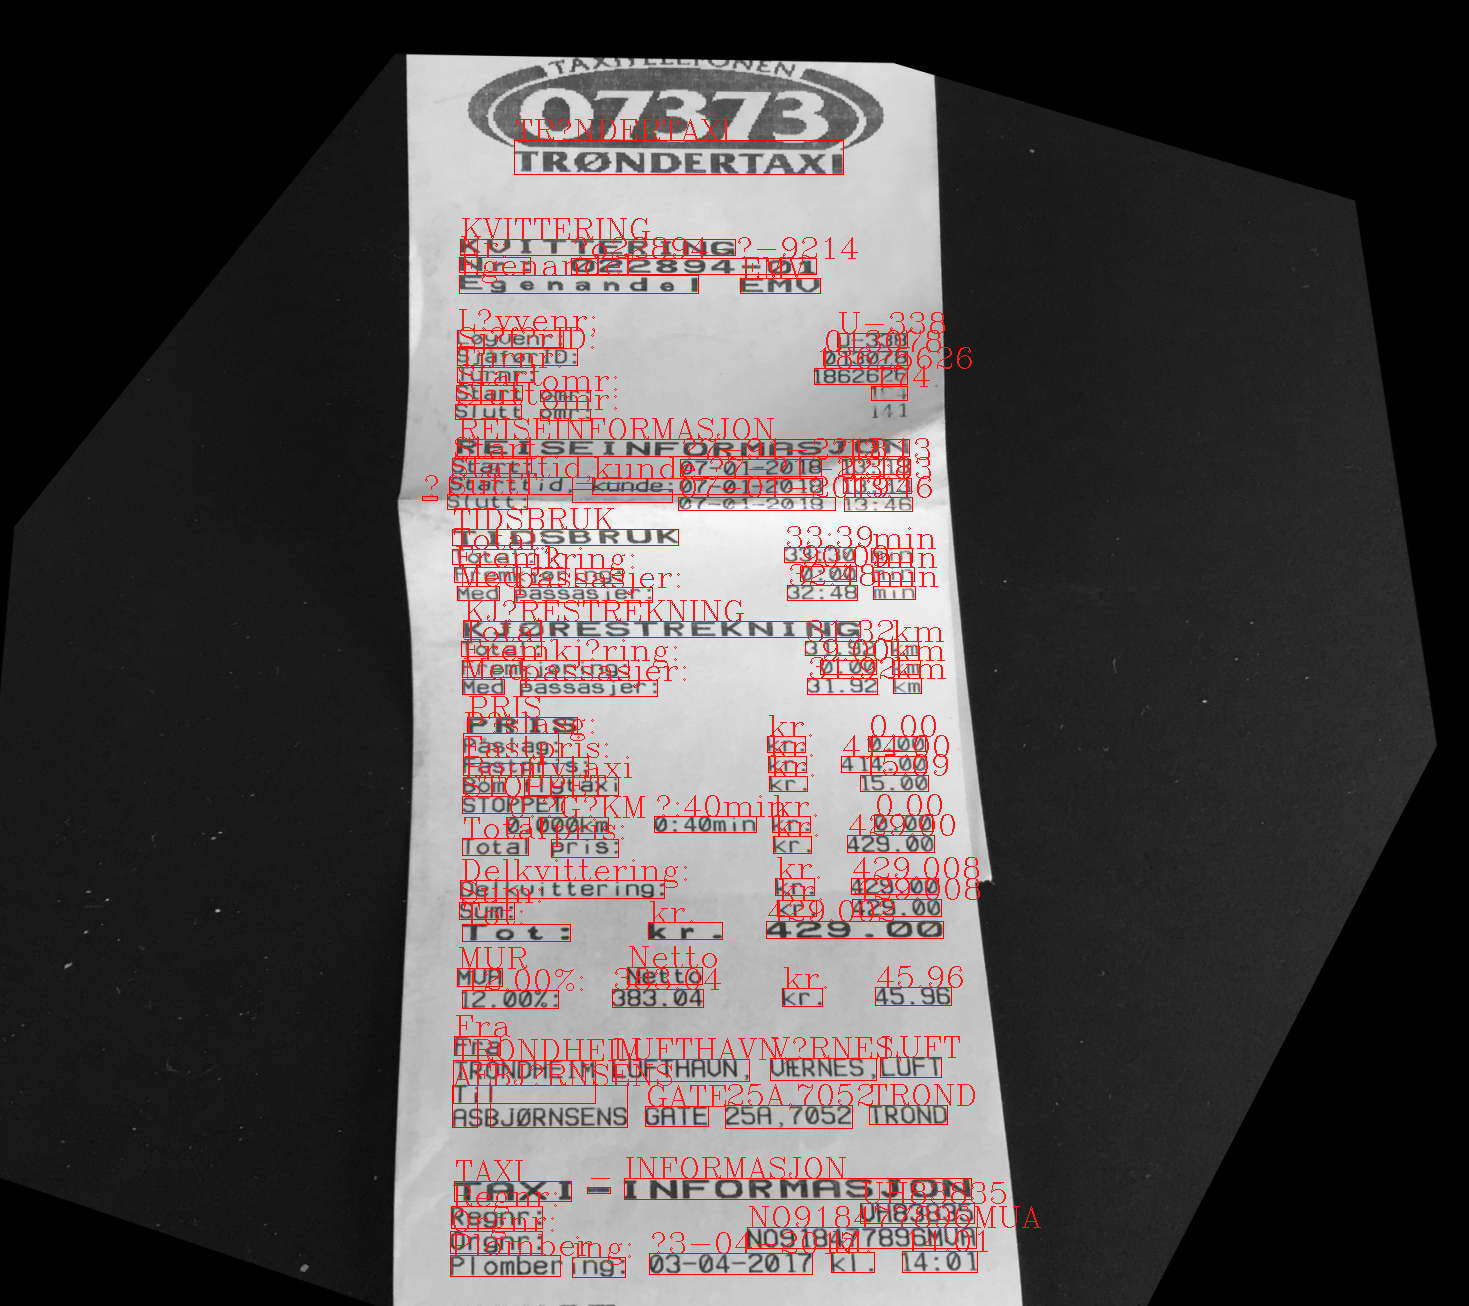
\includegraphics[width=0.6\textwidth]{Images/ocrtextboxes}}
    \caption{Extracted text in red, appearing over the place it has been extracted from}
    \label{fig:ocrtextboxes}
\end{figure}
\clearpage
Looking at figure~\ref{fig:ocrtextboxes}, the text seems to have been reasonably accurately extracted.
A date is then found using our regular expression for commonly used date formats.

\begin{figure}[h]
    \center{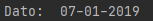
\includegraphics[width=0.5\textwidth]{Images/dateocr}}
    \caption{The date extracted from OCR output}
    \label{fig:dateocr}
\end{figure}

On further inspection, we can see that the date found in figure~\ref{fig:dateocr} does not match the date in
the image.
The date extracted from the OCR is from 2019, while the actual date should be 2018.
This means that the date that is given back to the API and back to the user, is not correct.
This example in particular highlights some issues with our implementation and will be discussed more in chapter 6.

The above example is a good indicator for what happens when the CNN correctly predicts the proper category, and when the image is readable by the OCR\@.
One of our categories of images were never readable by the OCR however.

\begin{figure}[h]
    \center{\includegraphics[width=1\textwidth]{Images/beforeafterflybuss}}
    \caption{Before and after pre-processing}
    \label{fig:beforeafterflybuss}
\end{figure}

\clearpage

\figurename{~\ref{fig:beforeafterflybuss}} shows the image as it is being sent from the user into our pipeline, and
after the OCR pre-processing.
The CNN made the correct prediction, as can be seen by the image not being rendered unusable by the de-skewing.


\begin{figure}[h]
    \center{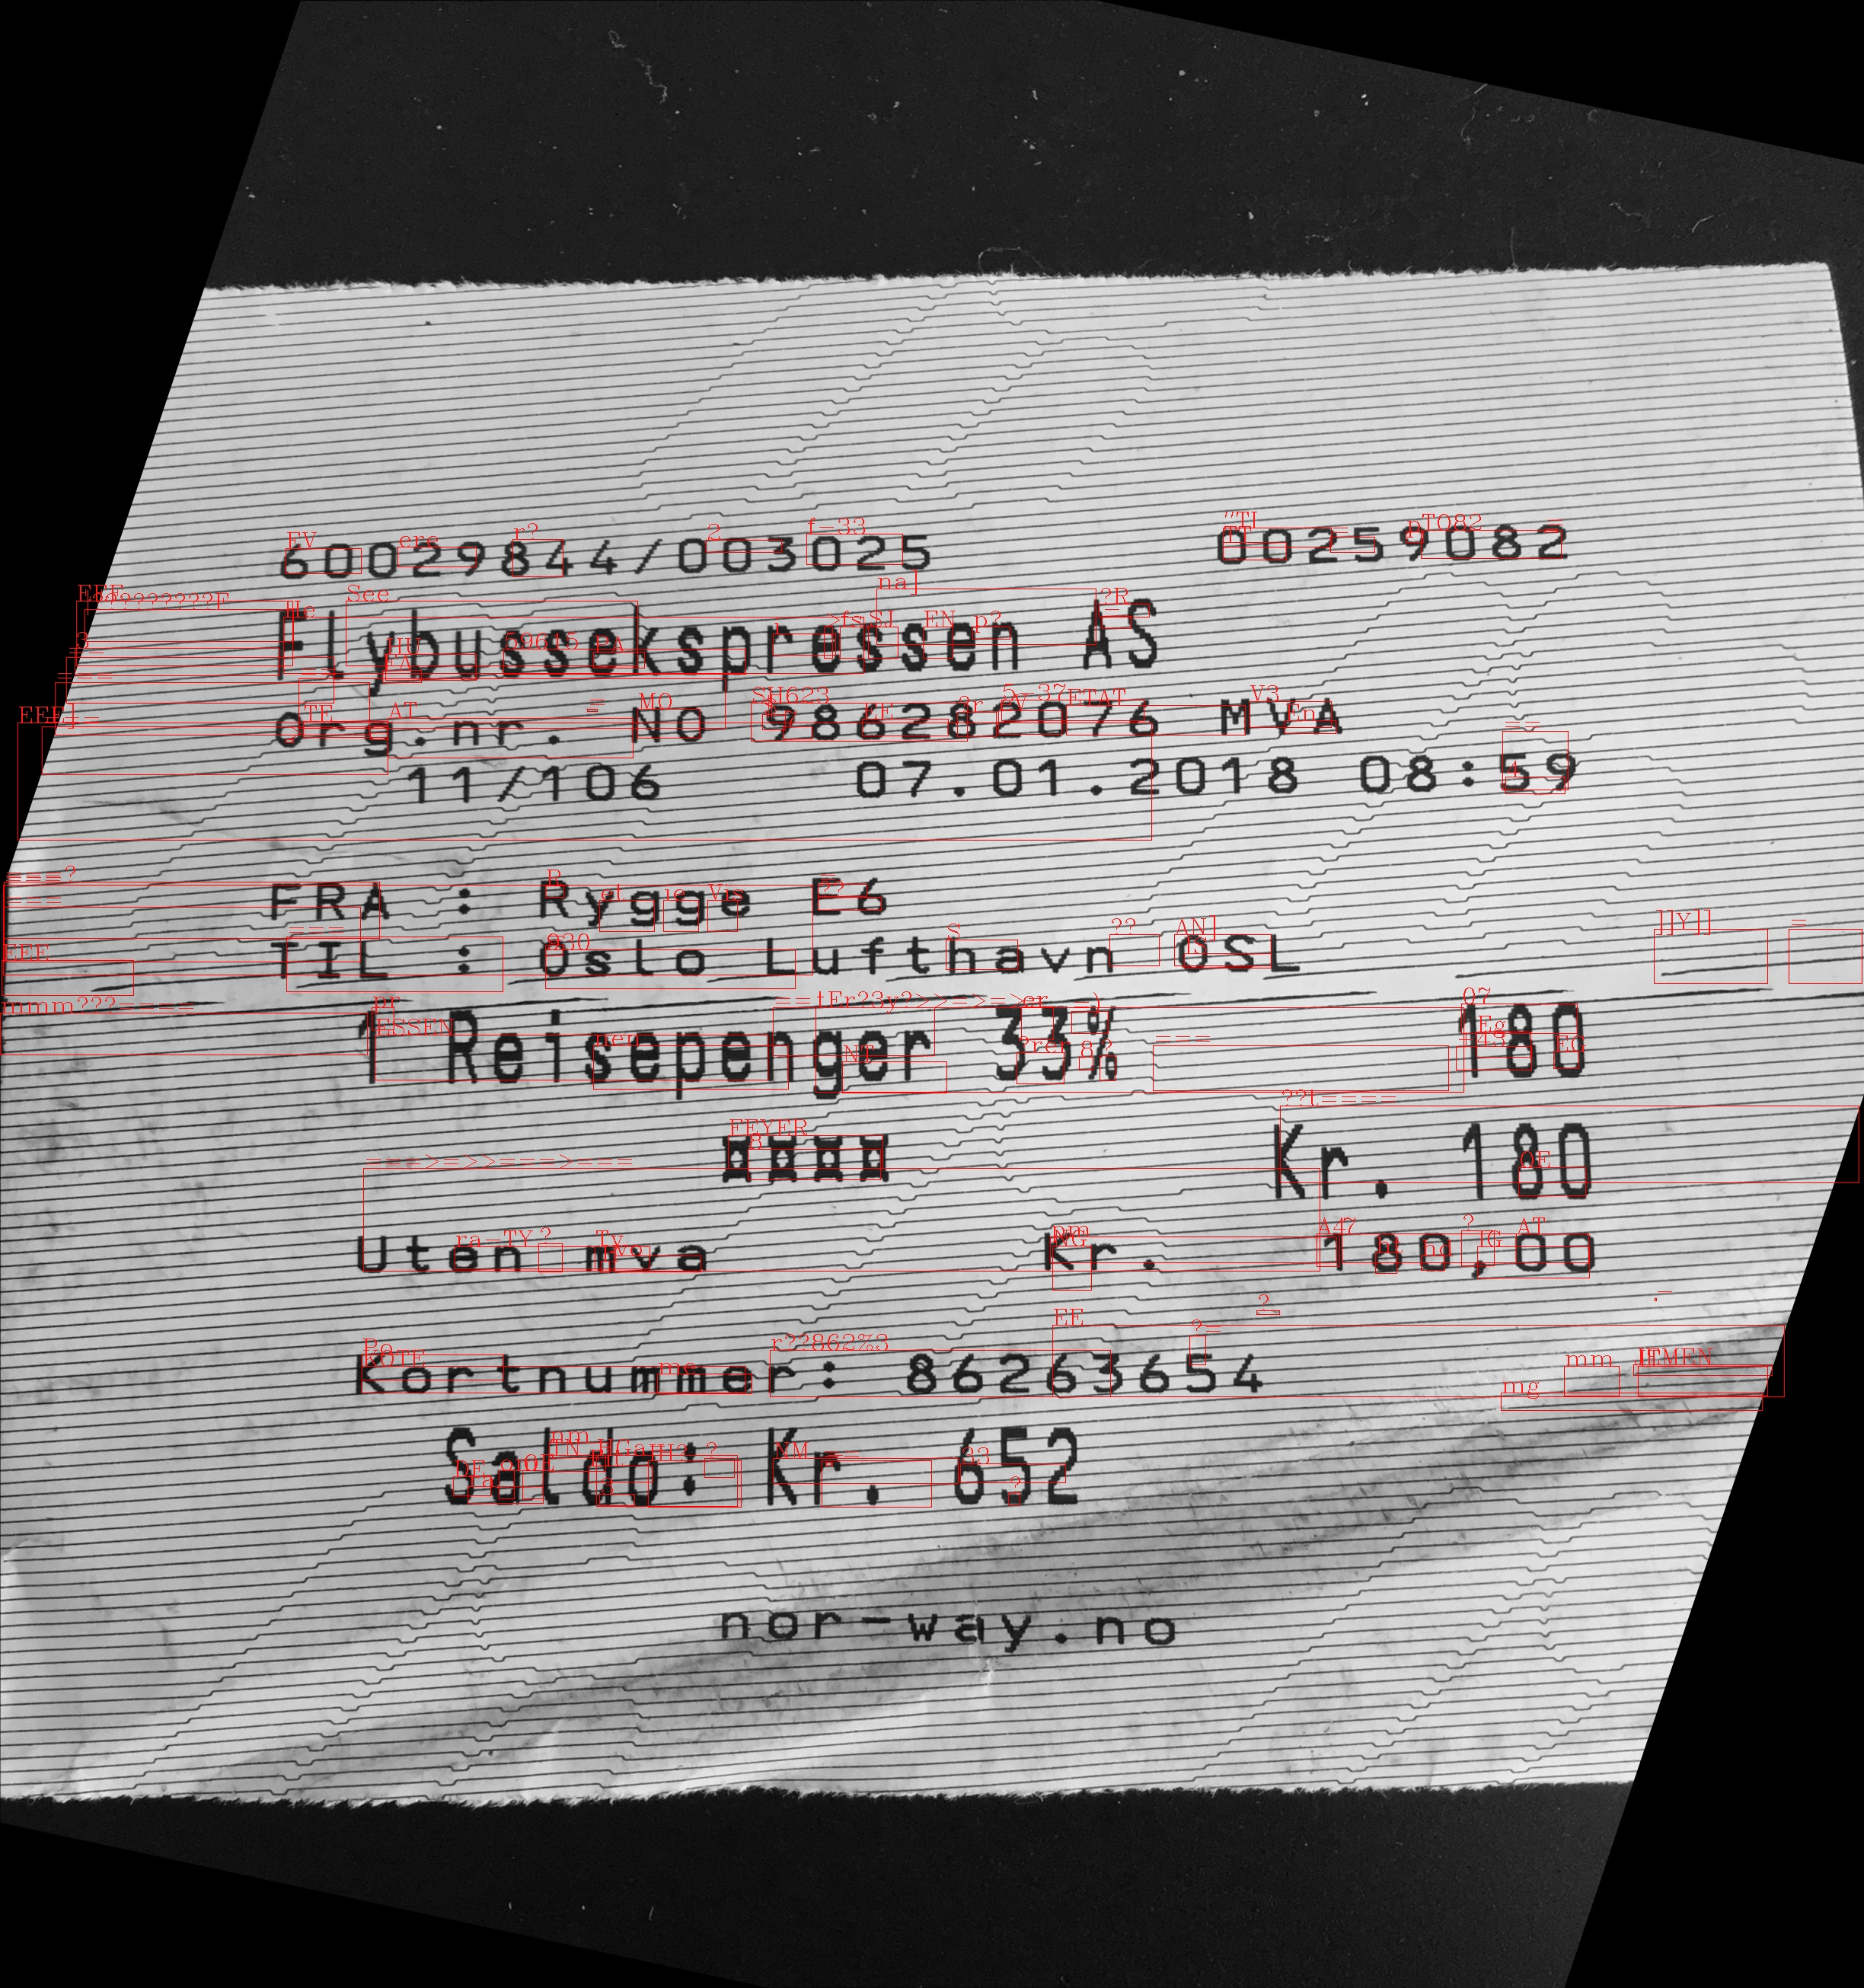
\includegraphics[width=0.7\textwidth]{Images/resultflybuss}}
    \caption{Extracted text in red, appearing over the place it has been extracted from}
    \label{fig:resultflybuss}
\end{figure}

Looking at the extracted text in figure~\ref{fig:resultflybuss}, it is apparent that the OCR did not
extract much useful information from the image.
Text is being found incorrectly along the edge of the receipt and in empty spaces in the receipt.
This is a recurring problem for receipts of this type, and will be discussed more in chapter 6.

\section{NER results}\label{sec:ner-results}
The text output from our OCR module is passed to our Spacy NER module for price extraction.
We were not able to extract any price information from Spacy's NER\@.
We will talk in debt about the price extraction in chapter~\ref{sec:price-extraction-with-spacy}.
\chapter{Discussion}
\label{ch:discussion}
\chapter{Conclusion}
\label{ch:conclusion}


\bibliographystyle{plain}   % Your preferred bibliogrphy style
\bibliography{main}       % DO NOT CHANGE, or substitute with another, or several, *.bib files

\printglossaries            % OPTIONAL, goes with \RequirePackage{glossaries}
\makeglossaries


\newglossaryentry{ML}
{
    name=Machine Learning,
    description={Machine Learning}
}

\newglossaryentry{API}
{
    name=Application Programming Interface,
    description={}
}
\newglossaryentry{HIOF}
{
    name=Østfold University College,
    description={}
}
\newglossaryentry{HRM}
{
    name=Human Resource Management,
    description={}
}
\newglossaryentry{OCR}
{
    name=Optical Character Recognition,
    description={}
}
\newglossaryentry{AWS}
{
    name=Amazon Web Services,
    description={}
}
 before

\appendix                   % OPTIONAL
\input{how-to}              % READ THIS CHAPTER: Sample code of everything you need and more :-)

\end{document}